\renewcommand{\theequation}{\theenumi}
\renewcommand{\thefigure}{\theenumi}
\renewcommand{\thetable}{\theenumi}
\begin{enumerate}[label=\thesection.\arabic*.,ref=\thesection.\theenumi]
\numberwithin{equation}{enumi}
\numberwithin{figure}{enumi}
\numberwithin{table}{enumi}

\item The probability that a given positive integer lying between 1 and 100 (both inclusive) is NOT divisible by 2,3 or 5 is \dots
\\
\solution
Table \ref{gate:11} summarizes the given information. 
\begin{table}[!ht]
    \begin{center}
        \renewcommand{\arraystretch}{2.5}
    \begin{tabular}{|c|c|c|}
    \hline
    Event & Definition & Probability  \\
    \hline
    A    & $n \equiv 0 \pmod{2}$  & $\cfrac{50}{100}$ \\ \hline
    B    & $n \equiv 0 \pmod{3}$ & $\cfrac{33}{100}$ \\ \hline
    C    & $n \equiv 0 \pmod{5}$  & $\cfrac{20}{100}$ \\ \hline
    AB   & $n \equiv 0 \pmod{6}$ & $\cfrac{16}{100}$ \\ \hline
    BC   & $n \equiv 0 \pmod{15}$ & $\cfrac{6}{100}$ \\ \hline
    AC   & $n \equiv 0 \pmod{10}$ & $\cfrac{10}{100}$ \\ \hline
    ABC  & $n \equiv 0 \pmod{30}$ & $\cfrac{3}{100}$ \\
    \hline
    \end{tabular}
    \renewcommand{\arraystretch}{1}
    \end{center}
    \caption{$1 \le n \le 100$}
    \label{gate:11}
    \end{table}
    %
%
\begin{multline}
\because     \pr{A+B+C} = \pr{A} + \pr{B} + \pr{C} \\- \pr{AB} - \pr{BC} \\- \pr{AC} + \pr{ABC}\label{Shurururururururu}    
\end{multline}

Substituting from Table \ref{gate:11} in \eqref{Shurururururururu},
\begin{multline}
    \pr{A+B+C} = \frac{50}{100} + \frac{33}{100} + \frac{20}{100} \\- \frac{16}{100} - \frac{6}{100} - \frac{10}{100} + \frac{3}{100} 
    \\
    = \frac{74}{100}
\end{multline}
Thus, the  required probability is
\begin{align}
    1 - \pr{A+B+C} = \frac{26}{100}
\end{align}

%
\item P and Q are considering to apply for a job. The probability that P applies for the job is $\dfrac{1}{4}$, the probability that P applies for the job given that Q applies for the job is $\dfrac{1}{2}$, and the probability that Q applies for the job given that P applies for the job is $\dfrac{1}{3}$. Then the probability that P does not apply for the job given that Q does not apply for the job is 

\begin{enumerate}
\begin{multicols}{4}
\setlength\itemsep{2em}

\item $
\dfrac{4}{5}
$

\item $
\dfrac{5}{6}
$

\item $
\dfrac{7}{8}
$

\item $
\dfrac{11}{12}
$

\end{multicols}
\end{enumerate}
\solution
The given information can be expressed as
\begin{align}
    \label{eq:axioms/2/given}
    \pr{P} &= \frac{1}{4} \\
    \pr{P|Q} &= \frac{1}{2}  = \frac{\pr{PQ}}{\pr{Q}}\\
    \pr{Q|P} &= \frac{1}{3}  =  \frac{\pr{PQ}}{\pr{P}}
    \end{align}
    which yields
    \begin{align}
        \label{eq:axioms/2/derived}
        \begin{split}
        \pr{PQ} &= \frac{1}{3} \times \frac{1}{4}  = \frac{1}{12}
        \\
        \pr{Q} &= \frac{\frac{1}{12}}{\frac{1}{2}} = \frac{1}{6}
        \end{split}
        \end{align}
    
The objective is to find
\begin{align}
    \pr{P^{\prime}|Q^{\prime}}
    \label{eq:axioms/2/tofind}
\end{align}
\eqref{eq:axioms/2/given} can be expressed as 
\begin{align}
    \pr{P^{\prime}|Q^{\prime}} &= \frac{\pr{P^{\prime}Q^{\prime}}}{\pr{Q^{\prime}}} 
\\
&= \frac{\pr{1 - \brak{P + Q}^{\prime}}}{\pr{Q^{\prime}}} 
\\
&= \frac{1 - \pr{P}-\pr{Q} +\pr{PQ}}{1 - \pr{Q}} 
   \label{2.0.19}   
    \end{align}
Substituting from     \eqref{eq:axioms/2/derived} and     \eqref{eq:axioms/2/given} in    \eqref{2.0.19},   
\begin{align}
    \pr{P^{\prime}|Q^{\prime}} = \frac{4}{5}
\end{align}


%
%
\item Out of 6 unbiased coins, 5 are tossed independently and they all result in heads. If the 6th coin is now independently tossed, the probability of getting head is:
\begin{enumerate}[label=(\alph*)]
\item 1
\item 0
\item $\frac{1}{2}$
\item $\frac{1}{6}$
\end{enumerate}
%
\solution
Define a random variable $X=\{0,1\}$ denoting the outcome of the toss of 6th coin with $X=0$ and $X=1$ representing tails and head respectively.Therefore,
\begin{align}
\pr{X=0} + \pr{X=1} &= 1\\
\pr{X=1} &= \frac{1}{2}
 \end{align}
 
Hence the correct answer is option $(\mathrm{c})$.

\item Two students are solving the same problem independently,if the probability of first one solves the problem is $\frac{3}{5}$ and the probability that the second one solves the problem is $\frac{4}{5}$ ,what is the probability that atleast one of them solves the problem?
\begin{enumerate}

\item $ \frac{17}{25}$\\
\item $\frac{19}{25}$\\
\item $ \frac{21}{25}$\\
\item $\frac{23}{25}$

\end{enumerate}
%
\solution
Let X,Y be two events representing solving the problem by students A,B respectively.\\
Given 
\begin{align}
    \pr{X}=\frac{3}{5}\label{june2018-18:eq:0.0.1}\\
    \pr{Y}=\frac{4}{5}\label{june2018-18:eq:0.0.2}
\end{align}
Since students solve the problem independently,So events X and Y are independent,
For independent events
\begin{align}
    \pr{XY}&=\pr{X}\times \pr{Y}
\intertext{from \eqref{june2018-18:eq:0.0.1} and \eqref{june2018-18:eq:0.0.2}}
    \pr{XY}&=\frac{3}{5}\times \frac{4}{5}\\
    \pr{XY}&=\frac{12}{25}\label{june2018-18:eq:0.0.5}
\end{align}
\\
\\Now we have to find probability of solving the problem by atleast one of them i.e $\pr{X+Y}$.\\
As,
\begin{align}
    \pr{X+Y}&=\pr{X}+\pr{Y}-\pr{XY}\\
\intertext{from \eqref{june2018-18:eq:0.0.1}, \eqref{june2018-18:eq:0.0.2}, \eqref{june2018-18:eq:0.0.5}}
\pr{X+Y}&=\frac{3}{5}+\frac{4}{5}-\frac{12}{25}\\
\pr{X+Y}&=\frac{23}{25}
\end{align}
Hence the required probability is $\frac{23}{25}$
%
\item Three types of components are used in electrical circuits 1, 2, 3 as shown below in the figure
\begin{figure}[h]
    \centering
    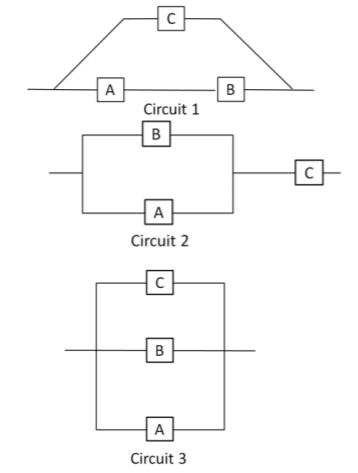
\includegraphics[width=\columnwidth]{solutions/2016/june/118/Figures/circuits.png}
    \caption{Figure}
    \label{fig:fig_label}
\end{figure}
%
\solution
For $q_1$, the truth table
\begin{table}[h]
    \centering
    \begin{tabular}{|c|c|c|c|}
    \hline
         $A$ & $B$ & $C$ & $(AB) + C$ \\
         \hline
         1 &1  & 0 &1\\\hline
         1&1&1&1\\\hline
         0&1&1&1\\\hline
         0&0&1&1\\\hline
         1&0&1&1\\
    \hline
    \end{tabular}
    \caption{Circuit 1 working}
    \label{june2016-118:tab:my_label}
\end{table}
Multiplying and adding probability for each case of $q_1$ gives us the value of $q_1$ as
\begin{align}
    q_1 = p^3-2p^2+1
\end{align}
For $q_2$, the truth table
\begin{table}[h]
    \centering
    \begin{tabular}{|c|c|c|c|}
    \hline
         $A$ & $B$ & $C$ & $(A+B)C$ \\
         \hline
         1&1&1&1\\ \hline
         1&0&1&1\\\hline
         0&1&1&1\\
    \hline
    \end{tabular}
    \caption{Circuit 2 working}
    \label{june2016-118:tab:table2}
\end{table}
Multiplying and adding probability for each case of $q_2$ gives us the value of $q_2$ as
\begin{align}
    q_2 = p^3-p^2-p+1
\end{align}
For $q_3$, the truth table
\begin{table}[h]
    \centering
    \begin{tabular}{|c|c|c|c|}
    \hline
         $A$ & $B$ & $C$ & $A + B + C$ \\
         \hline
         1&0&0&1\\\hline
         0&1&0&1\\\hline
         0&0&1&1\\\hline
         1&1&0&1\\\hline
         1&0&1&1\\\hline
         0&1&1&1\\\hline
         1&1&1&1\\
    \hline
    \end{tabular}
    \caption{Circuit 3 working}
    \label{june2016-118:tab:table3}
\end{table}
Multiplying and adding probability for each case of $q_3$ gives us the value of $q_3$ as
\begin{align}
    q_3 = 1-p^3
\end{align}
%%
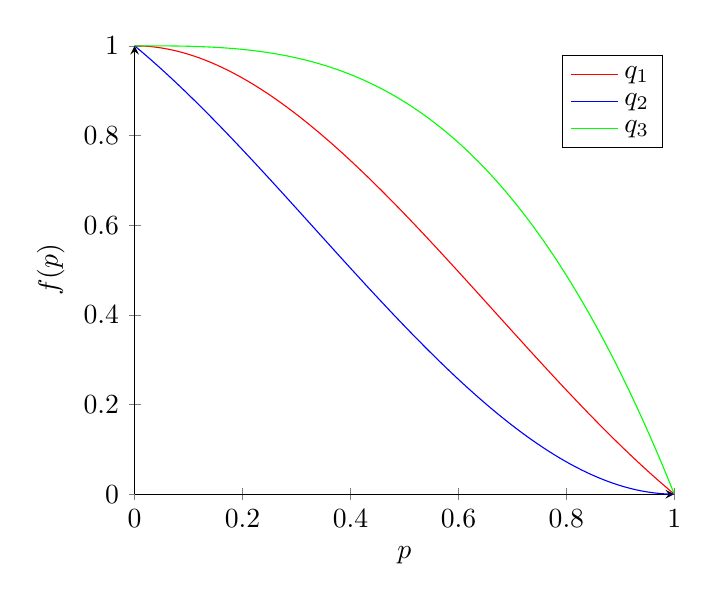
\begin{tikzpicture}
\begin{axis}[
    axis lines = left,
    xlabel = $p$,
    ylabel = {$f(p)$},
]
\addplot [
    domain=0:1, 
    samples=100, 
    color=red,
]
{x^3-2*x^2+1};
\addlegendentry{$q_1$}
\addplot [
    domain=0:1, 
    samples=100, 
    color=blue,
    ]
    {x^3-x^2-x+1};
\addlegendentry{$q_2$}
\addplot [
    domain=0:1, 
    samples=100, 
    color=green,
]
{1-x^3};
\addlegendentry{$q_3$}
\end{axis}
\end{tikzpicture}
\begin{align}
    \therefore q_3>q_1>q_2
\end{align}
Hence \textbf{Option 1} is correct
\end{enumerate}